\documentclass[1p]{elsarticle_modified}
%\bibliographystyle{elsarticle-num}

%\usepackage[colorlinks]{hyperref}
%\usepackage{abbrmath_seonhwa} %\Abb, \Ascr, \Acal ,\Abf, \Afrak
\usepackage{amsfonts}
\usepackage{amssymb}
\usepackage{amsmath}
\usepackage{amsthm}
\usepackage{scalefnt}
\usepackage{amsbsy}
\usepackage{kotex}
\usepackage{caption}
\usepackage{subfig}
\usepackage{color}
\usepackage{graphicx}
\usepackage{xcolor} %% white, black, red, green, blue, cyan, magenta, yellow
\usepackage{float}
\usepackage{setspace}
\usepackage{hyperref}

\usepackage{tikz}
\usetikzlibrary{arrows}

\usepackage{multirow}
\usepackage{array} % fixed length table
\usepackage{hhline}

%%%%%%%%%%%%%%%%%%%%%
\makeatletter
\renewcommand*\env@matrix[1][\arraystretch]{%
	\edef\arraystretch{#1}%
	\hskip -\arraycolsep
	\let\@ifnextchar\new@ifnextchar
	\array{*\c@MaxMatrixCols c}}
\makeatother %https://tex.stackexchange.com/questions/14071/how-can-i-increase-the-line-spacing-in-a-matrix
%%%%%%%%%%%%%%%

\usepackage[normalem]{ulem}

\newcommand{\msout}[1]{\ifmmode\text{\sout{\ensuremath{#1}}}\else\sout{#1}\fi}
%SOURCE: \msout is \stkout macro in https://tex.stackexchange.com/questions/20609/strikeout-in-math-mode

\newcommand{\cancel}[1]{
	\ifmmode
	{\color{red}\msout{#1}}
	\else
	{\color{red}\sout{#1}}
	\fi
}

\newcommand{\add}[1]{
	{\color{blue}\uwave{#1}}
}

\newcommand{\replace}[2]{
	\ifmmode
	{\color{red}\msout{#1}}{\color{blue}\uwave{#2}}
	\else
	{\color{red}\sout{#1}}{\color{blue}\uwave{#2}}
	\fi
}

\newcommand{\Sol}{\mathcal{S}} %segment
\newcommand{\D}{D} %diagram
\newcommand{\A}{\mathcal{A}} %arc


%%%%%%%%%%%%%%%%%%%%%%%%%%%%%5 test

\def\sl{\operatorname{\textup{SL}}(2,\Cbb)}
\def\psl{\operatorname{\textup{PSL}}(2,\Cbb)}
\def\quan{\mkern 1mu \triangleright \mkern 1mu}

\theoremstyle{definition}
\newtheorem{thm}{Theorem}[section]
\newtheorem{prop}[thm]{Proposition}
\newtheorem{lem}[thm]{Lemma}
\newtheorem{ques}[thm]{Question}
\newtheorem{cor}[thm]{Corollary}
\newtheorem{defn}[thm]{Definition}
\newtheorem{exam}[thm]{Example}
\newtheorem{rmk}[thm]{Remark}
\newtheorem{alg}[thm]{Algorithm}

\newcommand{\I}{\sqrt{-1}}
\begin{document}

%\begin{frontmatter}
%
%\title{Boundary parabolic representations of knots up to 8 crossings}
%
%%% Group authors per affiliation:
%\author{Yunhi Cho} 
%\address{Department of Mathematics, University of Seoul, Seoul, Korea}
%\ead{yhcho@uos.ac.kr}
%
%
%\author{Seonhwa Kim} %\fnref{s_kim}}
%\address{Center for Geometry and Physics, Institute for Basic Science, Pohang, 37673, Korea}
%\ead{ryeona17@ibs.re.kr}
%
%\author{Hyuk Kim}
%\address{Department of Mathematical Sciences, Seoul National University, Seoul 08826, Korea}
%\ead{hyukkim@snu.ac.kr}
%
%\author{Seokbeom Yoon}
%\address{Department of Mathematical Sciences, Seoul National University, Seoul, 08826,  Korea}
%\ead{sbyoon15@snu.ac.kr}
%
%\begin{abstract}
%We find all boundary parabolic representation of knots up to 8 crossings.
%
%\end{abstract}
%\begin{keyword}
%    \MSC[2010] 57M25 
%\end{keyword}
%
%\end{frontmatter}

%\linenumbers
%\tableofcontents
%
\newcommand\colored[1]{\textcolor{white}{\rule[-0.35ex]{0.8em}{1.4ex}}\kern-0.8em\color{red} #1}%
%\newcommand\colored[1]{\textcolor{white}{ #1}\kern-2.17ex	\textcolor{white}{ #1}\kern-1.81ex	\textcolor{white}{ #1}\kern-2.15ex\color{red}#1	}

{\Large $\underline{12n_{0300}~(K12n_{0300})}$}

\setlength{\tabcolsep}{10pt}
\renewcommand{\arraystretch}{1.6}
\vspace{1cm}\begin{tabular}{m{100pt}>{\centering\arraybackslash}m{274pt}}
\multirow{5}{120pt}{
	\centering
	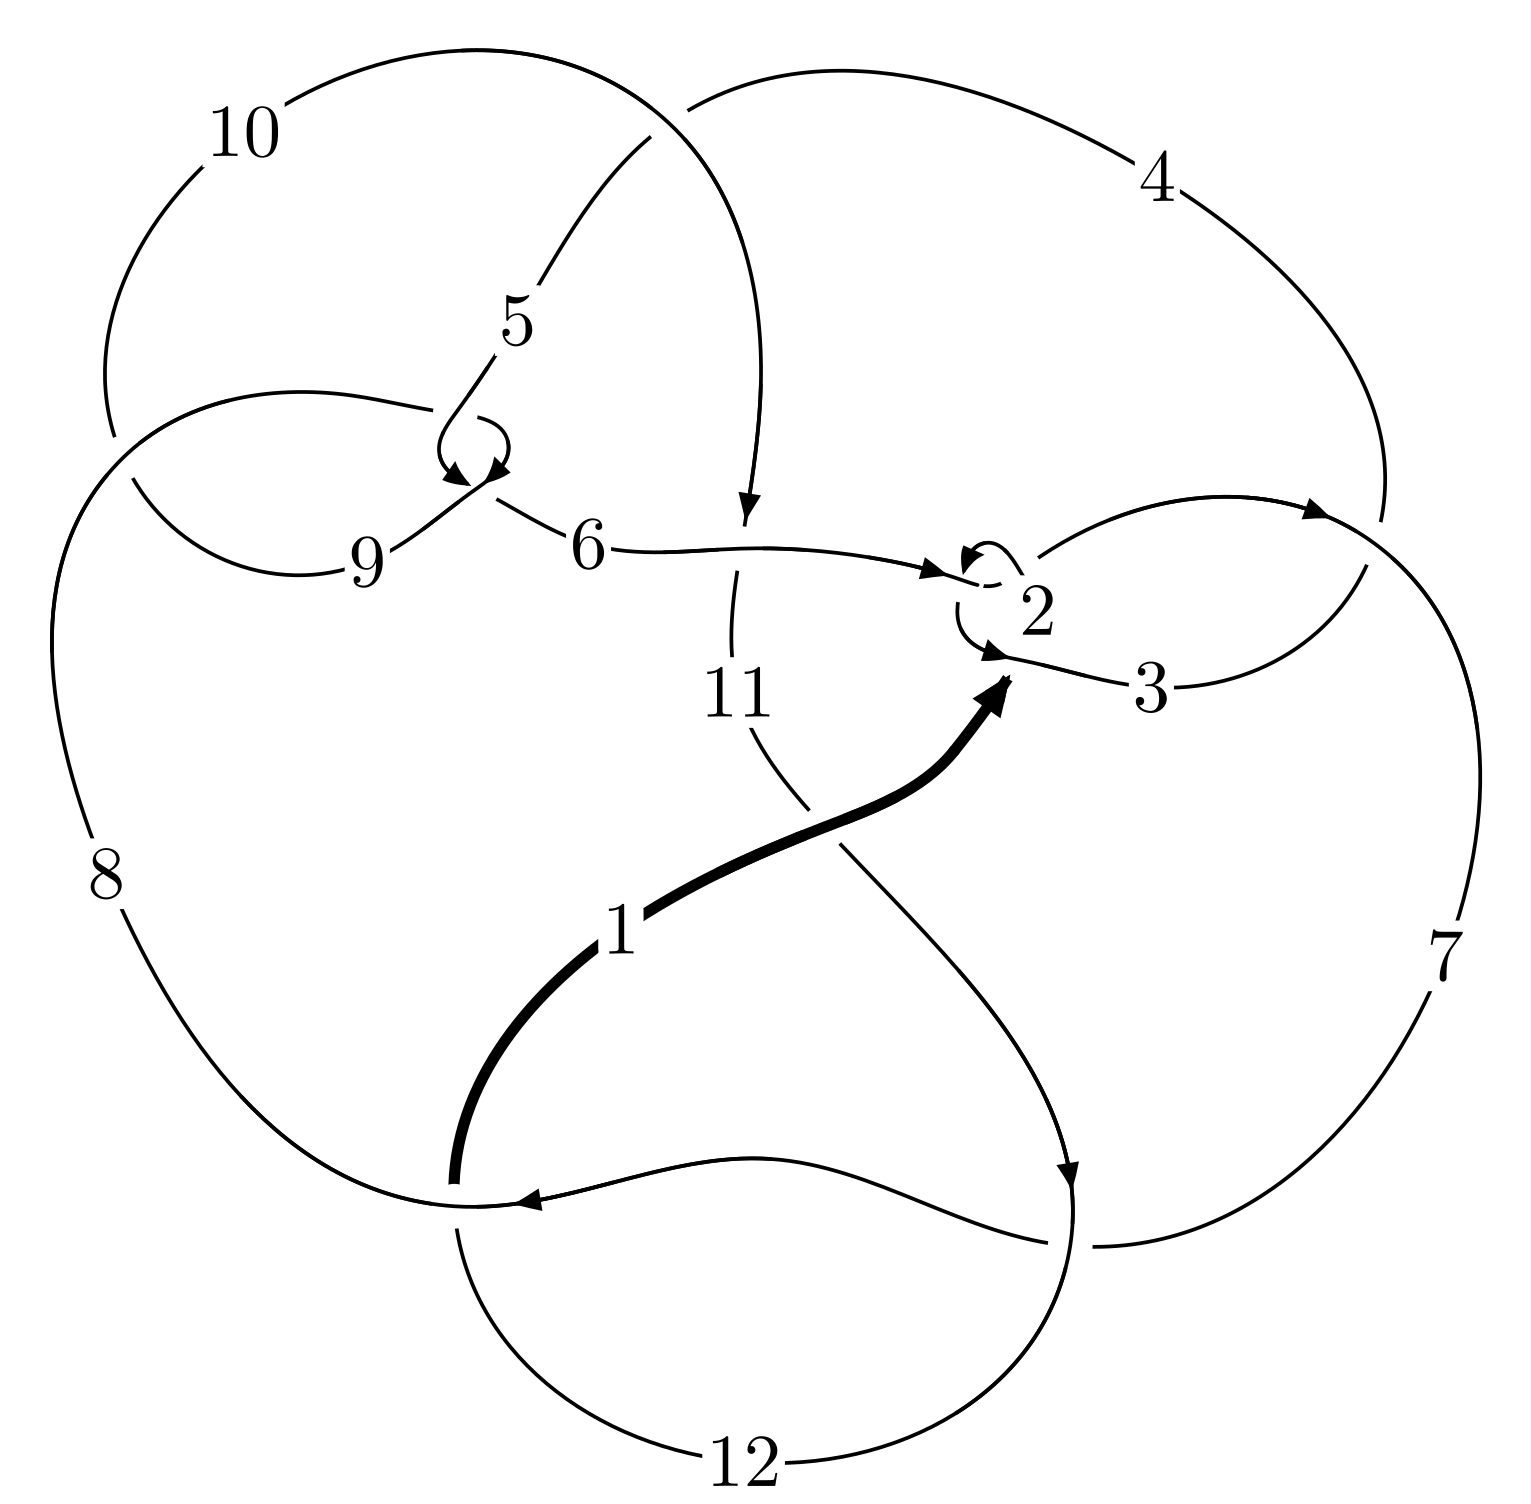
\includegraphics[width=112pt]{../../../GIT/diagram.site/Diagrams/png/2389_12n_0300.png}\\
\ \ \ A knot diagram\footnotemark}&
\allowdisplaybreaks
\textbf{Linearized knot diagam} \\
\cline{2-2}
 &
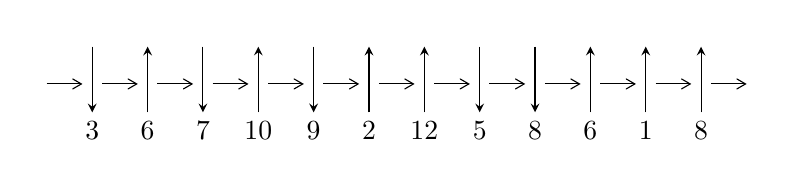
\begin{tikzpicture}[x=20pt, y=17pt]
	% nodes
	\node (C0) at (0, 0) {};
	\node (C1) at (1, 0) {};
	\node (C1U) at (1, +1) {};
	\node (C1D) at (1, -1) {3};

	\node (C2) at (2, 0) {};
	\node (C2U) at (2, +1) {};
	\node (C2D) at (2, -1) {6};

	\node (C3) at (3, 0) {};
	\node (C3U) at (3, +1) {};
	\node (C3D) at (3, -1) {7};

	\node (C4) at (4, 0) {};
	\node (C4U) at (4, +1) {};
	\node (C4D) at (4, -1) {10};

	\node (C5) at (5, 0) {};
	\node (C5U) at (5, +1) {};
	\node (C5D) at (5, -1) {9};

	\node (C6) at (6, 0) {};
	\node (C6U) at (6, +1) {};
	\node (C6D) at (6, -1) {2};

	\node (C7) at (7, 0) {};
	\node (C7U) at (7, +1) {};
	\node (C7D) at (7, -1) {12};

	\node (C8) at (8, 0) {};
	\node (C8U) at (8, +1) {};
	\node (C8D) at (8, -1) {5};

	\node (C9) at (9, 0) {};
	\node (C9U) at (9, +1) {};
	\node (C9D) at (9, -1) {8};

	\node (C10) at (10, 0) {};
	\node (C10U) at (10, +1) {};
	\node (C10D) at (10, -1) {6};

	\node (C11) at (11, 0) {};
	\node (C11U) at (11, +1) {};
	\node (C11D) at (11, -1) {1};

	\node (C12) at (12, 0) {};
	\node (C12U) at (12, +1) {};
	\node (C12D) at (12, -1) {8};
	\node (C13) at (13, 0) {};

	% arrows
	\draw[->,>={angle 60}]
	(C0) edge (C1) (C1) edge (C2) (C2) edge (C3) (C3) edge (C4) (C4) edge (C5) (C5) edge (C6) (C6) edge (C7) (C7) edge (C8) (C8) edge (C9) (C9) edge (C10) (C10) edge (C11) (C11) edge (C12) (C12) edge (C13) ;	\draw[->,>=stealth]
	(C1U) edge (C1D) (C2D) edge (C2U) (C3U) edge (C3D) (C4D) edge (C4U) (C5U) edge (C5D) (C6D) edge (C6U) (C7D) edge (C7U) (C8U) edge (C8D) (C9U) edge (C9D) (C10D) edge (C10U) (C11D) edge (C11U) (C12D) edge (C12U) ;
	\end{tikzpicture} \\
\hhline{~~} \\& 
\textbf{Solving Sequence} \\ \cline{2-2} 
 &
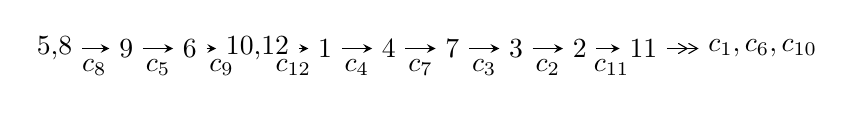
\begin{tikzpicture}[x=23pt, y=7pt]
	% node
	\node (A0) at (-1/8, 0) {5,8};
	\node (A1) at (1, 0) {9};
	\node (A2) at (2, 0) {6};
	\node (A3) at (49/16, 0) {10,12};
	\node (A4) at (33/8, 0) {1};
	\node (A5) at (41/8, 0) {4};
	\node (A6) at (49/8, 0) {7};
	\node (A7) at (57/8, 0) {3};
	\node (A8) at (65/8, 0) {2};
	\node (A9) at (73/8, 0) {11};
	\node (C1) at (1/2, -1) {$c_{8}$};
	\node (C2) at (3/2, -1) {$c_{5}$};
	\node (C3) at (5/2, -1) {$c_{9}$};
	\node (C4) at (29/8, -1) {$c_{12}$};
	\node (C5) at (37/8, -1) {$c_{4}$};
	\node (C6) at (45/8, -1) {$c_{7}$};
	\node (C7) at (53/8, -1) {$c_{3}$};
	\node (C8) at (61/8, -1) {$c_{2}$};
	\node (C9) at (69/8, -1) {$c_{11}$};
	\node (A10) at (11, 0) {$c_{1},c_{6},c_{10}$};

	% edge
	\draw[->,>=stealth]	
	(A0) edge (A1) (A1) edge (A2) (A2) edge (A3) (A3) edge (A4) (A4) edge (A5) (A5) edge (A6) (A6) edge (A7) (A7) edge (A8) (A8) edge (A9) ;
	\draw[->>,>={angle 60}]	
	(A9) edge (A10);
\end{tikzpicture} \\ 

\end{tabular} \\

\footnotetext{
The image of knot diagram is generated by the software ``\textbf{Draw programme}" developed by Andrew Bartholomew(\url{http://www.layer8.co.uk/maths/draw/index.htm\#Running-draw}), where we modified some parts for our purpose(\url{https://github.com/CATsTAILs/LinksPainter}).
}\phantom \\ \newline 
\centering \textbf{Ideals for irreducible components\footnotemark of $X_{\text{par}}$} 
 
\begin{align*}
I^u_{1}&=\langle 
-1.12945\times10^{24} u^{51}-1.35993\times10^{23} u^{50}+\cdots+4.17532\times10^{23} b+3.14183\times10^{24},\\
\phantom{I^u_{1}}&\phantom{= \langle  }6.04213\times10^{24} u^{51}-1.00196\times10^{24} u^{50}+\cdots+8.35063\times10^{23} a-2.70702\times10^{25},\;u^{52}- u^{51}+\cdots-4 u+4\rangle \\
I^u_{2}&=\langle 
b-1,\;u^3 a+4 u^2 a+2 u^3+2 a^2+5 u^2-2 u-6,\;u^4-2 u^2+2\rangle \\
\\
I^v_{1}&=\langle 
a,\;b+1,\;v^2- v+1\rangle \\
\end{align*}
\raggedright * 3 irreducible components of $\dim_{\mathbb{C}}=0$, with total 62 representations.\\
\footnotetext{All coefficients of polynomials are rational numbers. But the coefficients are sometimes approximated in decimal forms when there is not enough margin.}
\newpage
\renewcommand{\arraystretch}{1}
\centering \section*{I. $I^u_{1}= \langle -1.13\times10^{24} u^{51}-1.36\times10^{23} u^{50}+\cdots+4.18\times10^{23} b+3.14\times10^{24},\;6.04\times10^{24} u^{51}-1.00\times10^{24} u^{50}+\cdots+8.35\times10^{23} a-2.71\times10^{25},\;u^{52}- u^{51}+\cdots-4 u+4 \rangle$}
\flushleft \textbf{(i) Arc colorings}\\
\begin{tabular}{m{7pt} m{180pt} m{7pt} m{180pt} }
\flushright $a_{5}=$&$\begin{pmatrix}0\\u\end{pmatrix}$ \\
\flushright $a_{8}=$&$\begin{pmatrix}1\\0\end{pmatrix}$ \\
\flushright $a_{9}=$&$\begin{pmatrix}1\\u^2\end{pmatrix}$ \\
\flushright $a_{6}=$&$\begin{pmatrix}- u\\- u^3+u\end{pmatrix}$ \\
\flushright $a_{10}=$&$\begin{pmatrix}- u^2+1\\u^2\end{pmatrix}$ \\
\flushright $a_{12}=$&$\begin{pmatrix}-7.23554 u^{51}+1.19986 u^{50}+\cdots+2.91779 u+32.4170\\2.70507 u^{51}+0.325706 u^{50}+\cdots+4.65999 u-7.52477\end{pmatrix}$ \\
\flushright $a_{1}=$&$\begin{pmatrix}-4.53046 u^{51}+1.52557 u^{50}+\cdots+7.57778 u+24.8922\\2.70507 u^{51}+0.325706 u^{50}+\cdots+4.65999 u-7.52477\end{pmatrix}$ \\
\flushright $a_{4}=$&$\begin{pmatrix}- u^5+2 u^3- u\\u^5- u^3+u\end{pmatrix}$ \\
\flushright $a_{7}=$&$\begin{pmatrix}-1.40746 u^{51}+1.66161 u^{50}+\cdots+10.2665 u+13.5363\\-2.60824 u^{51}+0.294345 u^{50}+\cdots+0.650880 u+11.7241\end{pmatrix}$ \\
\flushright $a_{3}=$&$\begin{pmatrix}-10.3091 u^{51}+0.907634 u^{50}+\cdots-1.48074 u+45.2097\\1.04491 u^{51}+0.213681 u^{50}+\cdots+3.29442 u-2.54491\end{pmatrix}$ \\
\flushright $a_{2}=$&$\begin{pmatrix}-8.56753 u^{51}+0.985809 u^{50}+\cdots-0.320727 u+38.1282\\0.924923 u^{51}+0.0989994 u^{50}+\cdots+2.44711 u-2.74222\end{pmatrix}$ \\
\flushright $a_{11}=$&$\begin{pmatrix}u^6- u^4+1\\u^8-2 u^6+2 u^4\end{pmatrix}$\\&\end{tabular}
\flushleft \textbf{(ii) Obstruction class $= -1$}\\~\\
\flushleft \textbf{(iii) Cusp Shapes $= -\frac{749517475400009275308222}{208765812377423184830449} u^{51}+\frac{232040877417015531671918}{208765812377423184830449} u^{50}+\cdots-\frac{192808974281683631616226}{208765812377423184830449} u+\frac{4448015067704942886567602}{208765812377423184830449}$}\\~\\
\newpage\renewcommand{\arraystretch}{1}
\flushleft \textbf{(iv) u-Polynomials at the component}\newline \\
\begin{tabular}{m{50pt}|m{274pt}}
Crossings & \hspace{64pt}u-Polynomials at each crossing \\
\hline $$\begin{aligned}c_{1}\end{aligned}$$&$\begin{aligned}
&u^{52}+32 u^{51}+\cdots-74 u+25
\end{aligned}$\\
\hline $$\begin{aligned}c_{2},c_{6}\end{aligned}$$&$\begin{aligned}
&u^{52}-2 u^{51}+\cdots-8 u+5
\end{aligned}$\\
\hline $$\begin{aligned}c_{3}\end{aligned}$$&$\begin{aligned}
&u^{52}+2 u^{51}+\cdots-28 u+5
\end{aligned}$\\
\hline $$\begin{aligned}c_{4}\end{aligned}$$&$\begin{aligned}
&u^{52}+3 u^{51}+\cdots+460 u+76
\end{aligned}$\\
\hline $$\begin{aligned}c_{5},c_{8}\end{aligned}$$&$\begin{aligned}
&u^{52}+u^{51}+\cdots+4 u+4
\end{aligned}$\\
\hline $$\begin{aligned}c_{7},c_{12}\end{aligned}$$&$\begin{aligned}
&u^{52}-3 u^{51}+\cdots+9 u+1
\end{aligned}$\\
\hline $$\begin{aligned}c_{9}\end{aligned}$$&$\begin{aligned}
&u^{52}+31 u^{51}+\cdots+80 u+16
\end{aligned}$\\
\hline $$\begin{aligned}c_{10}\end{aligned}$$&$\begin{aligned}
&u^{52}- u^{51}+\cdots+1725404 u+2511892
\end{aligned}$\\
\hline $$\begin{aligned}c_{11}\end{aligned}$$&$\begin{aligned}
&u^{52}-13 u^{51}+\cdots-3 u+1
\end{aligned}$\\
\hline
\end{tabular}\\~\\
\newpage\renewcommand{\arraystretch}{1}
\flushleft \textbf{(v) Riley Polynomials at the component}\newline \\
\begin{tabular}{m{50pt}|m{274pt}}
Crossings & \hspace{64pt}Riley Polynomials at each crossing \\
\hline $$\begin{aligned}c_{1}\end{aligned}$$&$\begin{aligned}
&y^{52}-16 y^{51}+\cdots-48126 y+625
\end{aligned}$\\
\hline $$\begin{aligned}c_{2},c_{6}\end{aligned}$$&$\begin{aligned}
&y^{52}+32 y^{51}+\cdots-74 y+25
\end{aligned}$\\
\hline $$\begin{aligned}c_{3}\end{aligned}$$&$\begin{aligned}
&y^{52}-64 y^{51}+\cdots+326 y+25
\end{aligned}$\\
\hline $$\begin{aligned}c_{4}\end{aligned}$$&$\begin{aligned}
&y^{52}+61 y^{51}+\cdots-8528 y+5776
\end{aligned}$\\
\hline $$\begin{aligned}c_{5},c_{8}\end{aligned}$$&$\begin{aligned}
&y^{52}-31 y^{51}+\cdots-80 y+16
\end{aligned}$\\
\hline $$\begin{aligned}c_{7},c_{12}\end{aligned}$$&$\begin{aligned}
&y^{52}-13 y^{51}+\cdots-3 y+1
\end{aligned}$\\
\hline $$\begin{aligned}c_{9}\end{aligned}$$&$\begin{aligned}
&y^{52}-15 y^{51}+\cdots-3328 y+256
\end{aligned}$\\
\hline $$\begin{aligned}c_{10}\end{aligned}$$&$\begin{aligned}
&y^{52}+121 y^{51}+\cdots-158315434513616 y+6309601419664
\end{aligned}$\\
\hline $$\begin{aligned}c_{11}\end{aligned}$$&$\begin{aligned}
&y^{52}+67 y^{51}+\cdots+1413 y+1
\end{aligned}$\\
\hline
\end{tabular}\\~\\
\newpage\flushleft \textbf{(vi) Complex Volumes and Cusp Shapes}
$$\begin{array}{c|c|c}  
\text{Solutions to }I^u_{1}& \I (\text{vol} + \sqrt{-1}CS) & \text{Cusp shape}\\
 \hline 
\begin{aligned}
u &= -0.005040 + 0.945584 I \\
a &= -1.120450 - 0.773586 I \\
b &= \phantom{-}0.86363 + 1.15342 I\end{aligned}
 & -10.20250 - 1.40325 I & -0.753210 + 0.700768 I \\ \hline\begin{aligned}
u &= -0.005040 - 0.945584 I \\
a &= -1.120450 + 0.773586 I \\
b &= \phantom{-}0.86363 - 1.15342 I\end{aligned}
 & -10.20250 + 1.40325 I & -0.753210 - 0.700768 I \\ \hline\begin{aligned}
u &= \phantom{-}0.107775 + 0.930905 I \\
a &= -1.78820 - 0.36766 I \\
b &= \phantom{-}1.15916 + 0.95665 I\end{aligned}
 & -9.20690 + 9.05102 I & \phantom{-}0.53002 - 4.91799 I \\ \hline\begin{aligned}
u &= \phantom{-}0.107775 - 0.930905 I \\
a &= -1.78820 + 0.36766 I \\
b &= \phantom{-}1.15916 - 0.95665 I\end{aligned}
 & -9.20690 - 9.05102 I & \phantom{-}0.53002 + 4.91799 I \\ \hline\begin{aligned}
u &= \phantom{-}1.037360 + 0.298010 I \\
a &= \phantom{-}0.005298 + 0.154343 I \\
b &= \phantom{-}0.189541 + 0.596804 I\end{aligned}
 & -1.89487 - 1.25455 I & -1.66552 + 0.64316 I \\ \hline\begin{aligned}
u &= \phantom{-}1.037360 - 0.298010 I \\
a &= \phantom{-}0.005298 - 0.154343 I \\
b &= \phantom{-}0.189541 - 0.596804 I\end{aligned}
 & -1.89487 + 1.25455 I & -1.66552 - 0.64316 I \\ \hline\begin{aligned}
u &= -0.860656 + 0.321405 I \\
a &= -1.10246 + 2.20010 I \\
b &= \phantom{-}0.964482 + 0.321134 I\end{aligned}
 & \phantom{-}1.45283 + 3.79114 I & \phantom{-}3.95154 - 7.81429 I \\ \hline\begin{aligned}
u &= -0.860656 - 0.321405 I \\
a &= -1.10246 - 2.20010 I \\
b &= \phantom{-}0.964482 - 0.321134 I\end{aligned}
 & \phantom{-}1.45283 - 3.79114 I & \phantom{-}3.95154 + 7.81429 I \\ \hline\begin{aligned}
u &= \phantom{-}0.890991 + 0.199303 I \\
a &= \phantom{-}2.09257 - 0.24712 I \\
b &= -1.210700 - 0.125141 I\end{aligned}
 & \phantom{-}0.64653 - 3.09032 I & -0.45726 + 5.33318 I \\ \hline\begin{aligned}
u &= \phantom{-}0.890991 - 0.199303 I \\
a &= \phantom{-}2.09257 + 0.24712 I \\
b &= -1.210700 + 0.125141 I\end{aligned}
 & \phantom{-}0.64653 + 3.09032 I & -0.45726 - 5.33318 I\\
 \hline 
 \end{array}$$\newpage$$\begin{array}{c|c|c}  
\text{Solutions to }I^u_{1}& \I (\text{vol} + \sqrt{-1}CS) & \text{Cusp shape}\\
 \hline 
\begin{aligned}
u &= -0.056109 + 0.903857 I \\
a &= -1.370050 + 0.327066 I \\
b &= \phantom{-}0.983868 - 0.956085 I\end{aligned}
 & -5.60216 - 3.52882 I & \phantom{-}2.88518 + 2.10285 I \\ \hline\begin{aligned}
u &= -0.056109 - 0.903857 I \\
a &= -1.370050 - 0.327066 I \\
b &= \phantom{-}0.983868 + 0.956085 I\end{aligned}
 & -5.60216 + 3.52882 I & \phantom{-}2.88518 - 2.10285 I \\ \hline\begin{aligned}
u &= -0.993815 + 0.500766 I \\
a &= -1.65168 + 0.85430 I \\
b &= \phantom{-}0.815359 + 0.433581 I\end{aligned}
 & -0.20710 + 4.60134 I & \phantom{-}3.51877 - 6.93021 I \\ \hline\begin{aligned}
u &= -0.993815 - 0.500766 I \\
a &= -1.65168 - 0.85430 I \\
b &= \phantom{-}0.815359 - 0.433581 I\end{aligned}
 & -0.20710 - 4.60134 I & \phantom{-}3.51877 + 6.93021 I \\ \hline\begin{aligned}
u &= \phantom{-}0.824227 + 0.185520 I \\
a &= \phantom{-}0.19223 - 2.35056 I \\
b &= \phantom{-}0.870779 - 0.282220 I\end{aligned}
 & \phantom{-}0.857181 + 1.058030 I & \phantom{-}0.02381 + 1.93865 I \\ \hline\begin{aligned}
u &= \phantom{-}0.824227 - 0.185520 I \\
a &= \phantom{-}0.19223 + 2.35056 I \\
b &= \phantom{-}0.870779 + 0.282220 I\end{aligned}
 & \phantom{-}0.857181 - 1.058030 I & \phantom{-}0.02381 - 1.93865 I \\ \hline\begin{aligned}
u &= \phantom{-}0.448459 + 0.705408 I \\
a &= \phantom{-}1.35058 + 0.91047 I \\
b &= -0.593885 - 0.727712 I\end{aligned}
 & -1.53921 + 3.53715 I & \phantom{-}0.35654 - 4.05104 I \\ \hline\begin{aligned}
u &= \phantom{-}0.448459 - 0.705408 I \\
a &= \phantom{-}1.35058 - 0.91047 I \\
b &= -0.593885 + 0.727712 I\end{aligned}
 & -1.53921 - 3.53715 I & \phantom{-}0.35654 + 4.05104 I \\ \hline\begin{aligned}
u &= \phantom{-}1.017620 + 0.594178 I \\
a &= -1.99134 - 0.34195 I \\
b &= \phantom{-}0.772747 - 0.753613 I\end{aligned}
 & -3.15906 - 8.48239 I & \phantom{-0.000000 -}0. + 8.84514 I \\ \hline\begin{aligned}
u &= \phantom{-}1.017620 - 0.594178 I \\
a &= -1.99134 + 0.34195 I \\
b &= \phantom{-}0.772747 + 0.753613 I\end{aligned}
 & -3.15906 + 8.48239 I & \phantom{-0.000000 } 0. - 8.84514 I\\
 \hline 
 \end{array}$$\newpage$$\begin{array}{c|c|c}  
\text{Solutions to }I^u_{1}& \I (\text{vol} + \sqrt{-1}CS) & \text{Cusp shape}\\
 \hline 
\begin{aligned}
u &= \phantom{-}1.092570 + 0.474230 I \\
a &= -1.086010 - 0.165719 I \\
b &= \phantom{-}0.133855 - 0.142339 I\end{aligned}
 & -2.46320 - 1.67636 I & \phantom{-0.000000 } 0 \\ \hline\begin{aligned}
u &= \phantom{-}1.092570 - 0.474230 I \\
a &= -1.086010 + 0.165719 I \\
b &= \phantom{-}0.133855 + 0.142339 I\end{aligned}
 & -2.46320 + 1.67636 I & \phantom{-0.000000 } 0 \\ \hline\begin{aligned}
u &= -1.202650 + 0.144960 I \\
a &= -0.033095 - 0.253143 I \\
b &= \phantom{-}0.422921 - 1.043410 I\end{aligned}
 & -6.67676 - 1.37465 I & \phantom{-0.000000 } 0 \\ \hline\begin{aligned}
u &= -1.202650 - 0.144960 I \\
a &= -0.033095 + 0.253143 I \\
b &= \phantom{-}0.422921 + 1.043410 I\end{aligned}
 & -6.67676 + 1.37465 I & \phantom{-0.000000 } 0 \\ \hline\begin{aligned}
u &= \phantom{-}0.602001 + 0.506117 I \\
a &= \phantom{-}1.058240 - 0.518986 I \\
b &= -0.213970 + 0.512677 I\end{aligned}
 & -0.76208 - 1.83218 I & -0.54081 + 5.00541 I \\ \hline\begin{aligned}
u &= \phantom{-}0.602001 - 0.506117 I \\
a &= \phantom{-}1.058240 + 0.518986 I \\
b &= -0.213970 - 0.512677 I\end{aligned}
 & -0.76208 + 1.83218 I & -0.54081 - 5.00541 I \\ \hline\begin{aligned}
u &= -1.154940 + 0.386919 I \\
a &= -0.205260 - 0.701723 I \\
b &= -0.272895 - 0.607754 I\end{aligned}
 & -3.12200 + 5.95808 I & \phantom{-0.000000 } 0 \\ \hline\begin{aligned}
u &= -1.154940 - 0.386919 I \\
a &= -0.205260 + 0.701723 I \\
b &= -0.272895 + 0.607754 I\end{aligned}
 & -3.12200 - 5.95808 I & \phantom{-0.000000 } 0 \\ \hline\begin{aligned}
u &= \phantom{-}1.177630 + 0.344211 I \\
a &= -1.000060 - 0.963724 I \\
b &= \phantom{-}1.300120 - 0.319188 I\end{aligned}
 & -3.30400 - 3.98463 I & \phantom{-0.000000 } 0 \\ \hline\begin{aligned}
u &= \phantom{-}1.177630 - 0.344211 I \\
a &= -1.000060 + 0.963724 I \\
b &= \phantom{-}1.300120 + 0.319188 I\end{aligned}
 & -3.30400 + 3.98463 I & \phantom{-0.000000 } 0\\
 \hline 
 \end{array}$$\newpage$$\begin{array}{c|c|c}  
\text{Solutions to }I^u_{1}& \I (\text{vol} + \sqrt{-1}CS) & \text{Cusp shape}\\
 \hline 
\begin{aligned}
u &= -0.684305 + 0.345498 I \\
a &= \phantom{-}2.21655 - 0.15101 I \\
b &= -1.084480 + 0.183921 I\end{aligned}
 & \phantom{-}1.94565 - 0.69515 I & \phantom{-}5.57940 - 2.37743 I \\ \hline\begin{aligned}
u &= -0.684305 - 0.345498 I \\
a &= \phantom{-}2.21655 + 0.15101 I \\
b &= -1.084480 - 0.183921 I\end{aligned}
 & \phantom{-}1.94565 + 0.69515 I & \phantom{-}5.57940 + 2.37743 I \\ \hline\begin{aligned}
u &= -1.121360 + 0.516692 I \\
a &= -0.85701 + 1.13115 I \\
b &= \phantom{-}1.077300 - 0.327985 I\end{aligned}
 & -2.00208 + 3.98418 I & \phantom{-0.000000 } 0 \\ \hline\begin{aligned}
u &= -1.121360 - 0.516692 I \\
a &= -0.85701 - 1.13115 I \\
b &= \phantom{-}1.077300 + 0.327985 I\end{aligned}
 & -2.00208 - 3.98418 I & \phantom{-0.000000 } 0 \\ \hline\begin{aligned}
u &= -0.200571 + 0.677423 I \\
a &= \phantom{-}2.15588 + 0.29190 I \\
b &= -1.145000 - 0.260693 I\end{aligned}
 & \phantom{-}0.568023 + 0.563021 I & \phantom{-}1.46294 - 0.43596 I \\ \hline\begin{aligned}
u &= -0.200571 - 0.677423 I \\
a &= \phantom{-}2.15588 - 0.29190 I \\
b &= -1.145000 + 0.260693 I\end{aligned}
 & \phantom{-}0.568023 - 0.563021 I & \phantom{-}1.46294 + 0.43596 I \\ \hline\begin{aligned}
u &= -0.448987 + 0.506853 I \\
a &= \phantom{-}1.66812 - 0.26657 I \\
b &= -0.715266 + 0.202676 I\end{aligned}
 & \phantom{-}1.316970 - 0.435931 I & \phantom{-}7.52137 + 1.21169 I \\ \hline\begin{aligned}
u &= -0.448987 - 0.506853 I \\
a &= \phantom{-}1.66812 + 0.26657 I \\
b &= -0.715266 - 0.202676 I\end{aligned}
 & \phantom{-}1.316970 + 0.435931 I & \phantom{-}7.52137 - 1.21169 I \\ \hline\begin{aligned}
u &= \phantom{-}1.276530 + 0.439785 I \\
a &= -0.254365 + 0.161558 I \\
b &= -0.937038 - 1.050200 I\end{aligned}
 & -9.70077 - 1.19639 I & \phantom{-0.000000 } 0 \\ \hline\begin{aligned}
u &= \phantom{-}1.276530 - 0.439785 I \\
a &= -0.254365 - 0.161558 I \\
b &= -0.937038 + 1.050200 I\end{aligned}
 & -9.70077 + 1.19639 I & \phantom{-0.000000 } 0\\
 \hline 
 \end{array}$$\newpage$$\begin{array}{c|c|c}  
\text{Solutions to }I^u_{1}& \I (\text{vol} + \sqrt{-1}CS) & \text{Cusp shape}\\
 \hline 
\begin{aligned}
u &= -1.255740 + 0.501539 I \\
a &= \phantom{-}1.35852 - 1.19157 I \\
b &= -1.07227 - 0.96226 I\end{aligned}
 & -9.23940 + 8.57003 I & \phantom{-0.000000 } 0 \\ \hline\begin{aligned}
u &= -1.255740 - 0.501539 I \\
a &= \phantom{-}1.35852 + 1.19157 I \\
b &= -1.07227 + 0.96226 I\end{aligned}
 & -9.23940 - 8.57003 I & \phantom{-0.000000 } 0 \\ \hline\begin{aligned}
u &= \phantom{-}1.254730 + 0.531819 I \\
a &= \phantom{-}1.66106 + 1.24516 I \\
b &= -1.22933 + 0.93613 I\end{aligned}
 & -12.6957 - 14.3132 I & \phantom{-0.000000 } 0 \\ \hline\begin{aligned}
u &= \phantom{-}1.254730 - 0.531819 I \\
a &= \phantom{-}1.66106 - 1.24516 I \\
b &= -1.22933 - 0.93613 I\end{aligned}
 & -12.6957 + 14.3132 I & \phantom{-0.000000 } 0 \\ \hline\begin{aligned}
u &= -1.302310 + 0.406465 I \\
a &= \phantom{-}0.040415 - 0.203783 I \\
b &= -1.14144 + 1.05229 I\end{aligned}
 & -13.6366 - 4.3879 I & \phantom{-0.000000 } 0 \\ \hline\begin{aligned}
u &= -1.302310 - 0.406465 I \\
a &= \phantom{-}0.040415 + 0.203783 I \\
b &= -1.14144 - 1.05229 I\end{aligned}
 & -13.6366 + 4.3879 I & \phantom{-0.000000 } 0 \\ \hline\begin{aligned}
u &= -1.289050 + 0.482994 I \\
a &= -0.450643 - 0.411802 I \\
b &= -0.79762 + 1.24088 I\end{aligned}
 & -14.1610 + 6.4835 I & \phantom{-0.000000 } 0 \\ \hline\begin{aligned}
u &= -1.289050 - 0.482994 I \\
a &= -0.450643 + 0.411802 I \\
b &= -0.79762 - 1.24088 I\end{aligned}
 & -14.1610 - 6.4835 I & \phantom{-0.000000 } 0 \\ \hline\begin{aligned}
u &= \phantom{-}1.292070 + 0.476980 I \\
a &= \phantom{-}1.24277 + 0.80176 I \\
b &= -0.97197 + 1.17126 I\end{aligned}
 & -14.2080 - 3.6508 I & \phantom{-0.000000 } 0 \\ \hline\begin{aligned}
u &= \phantom{-}1.292070 - 0.476980 I \\
a &= \phantom{-}1.24277 - 0.80176 I \\
b &= -0.97197 - 1.17126 I\end{aligned}
 & -14.2080 + 3.6508 I & \phantom{-0.000000 } 0\\
 \hline 
 \end{array}$$\newpage$$\begin{array}{c|c|c}  
\text{Solutions to }I^u_{1}& \I (\text{vol} + \sqrt{-1}CS) & \text{Cusp shape}\\
 \hline 
\begin{aligned}
u &= \phantom{-}0.053574 + 0.599232 I \\
a &= \phantom{-}0.868407 - 0.120577 I \\
b &= \phantom{-}0.332102 - 0.211608 I\end{aligned}
 & \phantom{-}0.20589 - 2.30089 I & -0.01971 + 3.72749 I \\ \hline\begin{aligned}
u &= \phantom{-}0.053574 - 0.599232 I \\
a &= \phantom{-}0.868407 + 0.120577 I \\
b &= \phantom{-}0.332102 + 0.211608 I\end{aligned}
 & \phantom{-}0.20589 + 2.30089 I & -0.01971 - 3.72749 I\\
 \hline 
 \end{array}$$\newpage\newpage\renewcommand{\arraystretch}{1}
\centering \section*{II. $I^u_{2}= \langle b-1,\;u^3 a+4 u^2 a+2 u^3+2 a^2+5 u^2-2 u-6,\;u^4-2 u^2+2 \rangle$}
\flushleft \textbf{(i) Arc colorings}\\
\begin{tabular}{m{7pt} m{180pt} m{7pt} m{180pt} }
\flushright $a_{5}=$&$\begin{pmatrix}0\\u\end{pmatrix}$ \\
\flushright $a_{8}=$&$\begin{pmatrix}1\\0\end{pmatrix}$ \\
\flushright $a_{9}=$&$\begin{pmatrix}1\\u^2\end{pmatrix}$ \\
\flushright $a_{6}=$&$\begin{pmatrix}- u\\- u^3+u\end{pmatrix}$ \\
\flushright $a_{10}=$&$\begin{pmatrix}- u^2+1\\u^2\end{pmatrix}$ \\
\flushright $a_{12}=$&$\begin{pmatrix}a\\1\end{pmatrix}$ \\
\flushright $a_{1}=$&$\begin{pmatrix}a+1\\1\end{pmatrix}$ \\
\flushright $a_{4}=$&$\begin{pmatrix}u\\u^3- u\end{pmatrix}$ \\
\flushright $a_{7}=$&$\begin{pmatrix}a+1\\1\end{pmatrix}$ \\
\flushright $a_{3}=$&$\begin{pmatrix}\frac{3}{2} u^3+a u+u^2+a+u\\u^3 a+2 u^3- a u-3 u\end{pmatrix}$ \\
\flushright $a_{2}=$&$\begin{pmatrix}u^2 a+\frac{3}{2} u^3+a u+u^2- a-2\\u^3 a- u^2 a+u^3- a u-2 u^2-2 u+2\end{pmatrix}$ \\
\flushright $a_{11}=$&$\begin{pmatrix}-1\\0\end{pmatrix}$\\&\end{tabular}
\flushleft \textbf{(ii) Obstruction class $= 1$}\\~\\
\flushleft \textbf{(iii) Cusp Shapes $= 4 u^3 a+4 u^3-4 a u+4 u^2-8 u-4$}\\~\\
\newpage\renewcommand{\arraystretch}{1}
\flushleft \textbf{(iv) u-Polynomials at the component}\newline \\
\begin{tabular}{m{50pt}|m{274pt}}
Crossings & \hspace{64pt}u-Polynomials at each crossing \\
\hline $$\begin{aligned}c_{1},c_{2}\end{aligned}$$&$\begin{aligned}
&(u^2- u+1)^4
\end{aligned}$\\
\hline $$\begin{aligned}c_{3},c_{6}\end{aligned}$$&$\begin{aligned}
&(u^2+u+1)^4
\end{aligned}$\\
\hline $$\begin{aligned}c_{4},c_{10}\end{aligned}$$&$\begin{aligned}
&(u^4+2 u^2+2)^2
\end{aligned}$\\
\hline $$\begin{aligned}c_{5},c_{8}\end{aligned}$$&$\begin{aligned}
&(u^4-2 u^2+2)^2
\end{aligned}$\\
\hline $$\begin{aligned}c_{7}\end{aligned}$$&$\begin{aligned}
&(u-1)^8
\end{aligned}$\\
\hline $$\begin{aligned}c_{9}\end{aligned}$$&$\begin{aligned}
&(u^2+2 u+2)^4
\end{aligned}$\\
\hline $$\begin{aligned}c_{11},c_{12}\end{aligned}$$&$\begin{aligned}
&(u+1)^8
\end{aligned}$\\
\hline
\end{tabular}\\~\\
\newpage\renewcommand{\arraystretch}{1}
\flushleft \textbf{(v) Riley Polynomials at the component}\newline \\
\begin{tabular}{m{50pt}|m{274pt}}
Crossings & \hspace{64pt}Riley Polynomials at each crossing \\
\hline $$\begin{aligned}c_{1},c_{2},c_{3}\\c_{6}\end{aligned}$$&$\begin{aligned}
&(y^2+y+1)^4
\end{aligned}$\\
\hline $$\begin{aligned}c_{4},c_{10}\end{aligned}$$&$\begin{aligned}
&(y^2+2 y+2)^4
\end{aligned}$\\
\hline $$\begin{aligned}c_{5},c_{8}\end{aligned}$$&$\begin{aligned}
&(y^2-2 y+2)^4
\end{aligned}$\\
\hline $$\begin{aligned}c_{7},c_{11},c_{12}\end{aligned}$$&$\begin{aligned}
&(y-1)^8
\end{aligned}$\\
\hline $$\begin{aligned}c_{9}\end{aligned}$$&$\begin{aligned}
&(y^2+4)^4
\end{aligned}$\\
\hline
\end{tabular}\\~\\
\newpage\flushleft \textbf{(vi) Complex Volumes and Cusp Shapes}
$$\begin{array}{c|c|c}  
\text{Solutions to }I^u_{2}& \I (\text{vol} + \sqrt{-1}CS) & \text{Cusp shape}\\
 \hline 
\begin{aligned}
u &= \phantom{-}1.098680 + 0.455090 I \\
a &= -0.48809 - 1.66713 I \\
b &= \phantom{-}1.00000\phantom{ +0.000000I}\end{aligned}
 & -0.82247 - 5.69375 I & \phantom{-}2.00000 + 7.46410 I \\ \hline\begin{aligned}
u &= \phantom{-}1.098680 + 0.455090 I \\
a &= -1.83370 - 1.10976 I \\
b &= \phantom{-}1.00000\phantom{ +0.000000I}\end{aligned}
 & -0.82247 - 1.63398 I & \phantom{-}2.00000 + 0.53590 I \\ \hline\begin{aligned}
u &= \phantom{-}1.098680 - 0.455090 I \\
a &= -0.48809 + 1.66713 I \\
b &= \phantom{-}1.00000\phantom{ +0.000000I}\end{aligned}
 & -0.82247 + 5.69375 I & \phantom{-}2.00000 - 7.46410 I \\ \hline\begin{aligned}
u &= \phantom{-}1.098680 - 0.455090 I \\
a &= -1.83370 + 1.10976 I \\
b &= \phantom{-}1.00000\phantom{ +0.000000I}\end{aligned}
 & -0.82247 + 1.63398 I & \phantom{-}2.00000 - 0.53590 I \\ \hline\begin{aligned}
u &= -1.098680 + 0.455090 I \\
a &= -0.166298 + 0.890241 I \\
b &= \phantom{-}1.00000\phantom{ +0.000000I}\end{aligned}
 & -0.82247 + 1.63398 I & \phantom{-}2.00000 - 0.53590 I \\ \hline\begin{aligned}
u &= -1.098680 + 0.455090 I \\
a &= -1.51191 + 0.33287 I \\
b &= \phantom{-}1.00000\phantom{ +0.000000I}\end{aligned}
 & -0.82247 + 5.69375 I & \phantom{-}2.00000 - 7.46410 I \\ \hline\begin{aligned}
u &= -1.098680 - 0.455090 I \\
a &= -0.166298 - 0.890241 I \\
b &= \phantom{-}1.00000\phantom{ +0.000000I}\end{aligned}
 & -0.82247 - 1.63398 I & \phantom{-}2.00000 + 0.53590 I \\ \hline\begin{aligned}
u &= -1.098680 - 0.455090 I \\
a &= -1.51191 - 0.33287 I \\
b &= \phantom{-}1.00000\phantom{ +0.000000I}\end{aligned}
 & -0.82247 - 5.69375 I & \phantom{-}2.00000 + 7.46410 I\\
 \hline 
 \end{array}$$\newpage\newpage\renewcommand{\arraystretch}{1}
\centering \section*{III. $I^v_{1}= \langle a,\;b+1,\;v^2- v+1 \rangle$}
\flushleft \textbf{(i) Arc colorings}\\
\begin{tabular}{m{7pt} m{180pt} m{7pt} m{180pt} }
\flushright $a_{5}=$&$\begin{pmatrix}v\\0\end{pmatrix}$ \\
\flushright $a_{8}=$&$\begin{pmatrix}1\\0\end{pmatrix}$ \\
\flushright $a_{9}=$&$\begin{pmatrix}1\\0\end{pmatrix}$ \\
\flushright $a_{6}=$&$\begin{pmatrix}v\\0\end{pmatrix}$ \\
\flushright $a_{10}=$&$\begin{pmatrix}1\\0\end{pmatrix}$ \\
\flushright $a_{12}=$&$\begin{pmatrix}0\\-1\end{pmatrix}$ \\
\flushright $a_{1}=$&$\begin{pmatrix}-1\\-1\end{pmatrix}$ \\
\flushright $a_{4}=$&$\begin{pmatrix}v\\0\end{pmatrix}$ \\
\flushright $a_{7}=$&$\begin{pmatrix}1\\1\end{pmatrix}$ \\
\flushright $a_{3}=$&$\begin{pmatrix}0\\- v\end{pmatrix}$ \\
\flushright $a_{2}=$&$\begin{pmatrix}-1\\- v\end{pmatrix}$ \\
\flushright $a_{11}=$&$\begin{pmatrix}1\\0\end{pmatrix}$\\&\end{tabular}
\flushleft \textbf{(ii) Obstruction class $= 1$}\\~\\
\flushleft \textbf{(iii) Cusp Shapes $= 4 v+4$}\\~\\
\newpage\renewcommand{\arraystretch}{1}
\flushleft \textbf{(iv) u-Polynomials at the component}\newline \\
\begin{tabular}{m{50pt}|m{274pt}}
Crossings & \hspace{64pt}u-Polynomials at each crossing \\
\hline $$\begin{aligned}c_{1},c_{3},c_{6}\end{aligned}$$&$\begin{aligned}
&u^2- u+1
\end{aligned}$\\
\hline $$\begin{aligned}c_{2}\end{aligned}$$&$\begin{aligned}
&u^2+u+1
\end{aligned}$\\
\hline $$\begin{aligned}c_{4},c_{5},c_{8}\\c_{9},c_{10}\end{aligned}$$&$\begin{aligned}
&u^2
\end{aligned}$\\
\hline $$\begin{aligned}c_{7},c_{11}\end{aligned}$$&$\begin{aligned}
&(u+1)^2
\end{aligned}$\\
\hline $$\begin{aligned}c_{12}\end{aligned}$$&$\begin{aligned}
&(u-1)^2
\end{aligned}$\\
\hline
\end{tabular}\\~\\
\newpage\renewcommand{\arraystretch}{1}
\flushleft \textbf{(v) Riley Polynomials at the component}\newline \\
\begin{tabular}{m{50pt}|m{274pt}}
Crossings & \hspace{64pt}Riley Polynomials at each crossing \\
\hline $$\begin{aligned}c_{1},c_{2},c_{3}\\c_{6}\end{aligned}$$&$\begin{aligned}
&y^2+y+1
\end{aligned}$\\
\hline $$\begin{aligned}c_{4},c_{5},c_{8}\\c_{9},c_{10}\end{aligned}$$&$\begin{aligned}
&y^2
\end{aligned}$\\
\hline $$\begin{aligned}c_{7},c_{11},c_{12}\end{aligned}$$&$\begin{aligned}
&(y-1)^2
\end{aligned}$\\
\hline
\end{tabular}\\~\\
\newpage\flushleft \textbf{(vi) Complex Volumes and Cusp Shapes}
$$\begin{array}{c|c|c}  
\text{Solutions to }I^v_{1}& \I (\text{vol} + \sqrt{-1}CS) & \text{Cusp shape}\\
 \hline 
\begin{aligned}
v &= \phantom{-}0.500000 + 0.866025 I \\
a &= \phantom{-0.000000 } 0 \\
b &= -1.00000\phantom{ +0.000000I}\end{aligned}
 & \phantom{-}1.64493 - 2.02988 I & \phantom{-}6.00000 + 3.46410 I \\ \hline\begin{aligned}
v &= \phantom{-}0.500000 - 0.866025 I \\
a &= \phantom{-0.000000 } 0 \\
b &= -1.00000\phantom{ +0.000000I}\end{aligned}
 & \phantom{-}1.64493 + 2.02988 I & \phantom{-}6.00000 - 3.46410 I\\
 \hline 
 \end{array}$$\newpage
\newpage\renewcommand{\arraystretch}{1}
\centering \section*{ IV. u-Polynomials}
\begin{tabular}{m{50pt}|m{274pt}}
Crossings & \hspace{64pt}u-Polynomials at each crossing \\
\hline $$\begin{aligned}c_{1}\end{aligned}$$&$\begin{aligned}
&((u^2- u+1)^5)(u^{52}+32 u^{51}+\cdots-74 u+25)
\end{aligned}$\\
\hline $$\begin{aligned}c_{2}\end{aligned}$$&$\begin{aligned}
&((u^2- u+1)^4)(u^2+u+1)(u^{52}-2 u^{51}+\cdots-8 u+5)
\end{aligned}$\\
\hline $$\begin{aligned}c_{3}\end{aligned}$$&$\begin{aligned}
&(u^2- u+1)(u^2+u+1)^4(u^{52}+2 u^{51}+\cdots-28 u+5)
\end{aligned}$\\
\hline $$\begin{aligned}c_{4}\end{aligned}$$&$\begin{aligned}
&u^2(u^4+2 u^2+2)^2(u^{52}+3 u^{51}+\cdots+460 u+76)
\end{aligned}$\\
\hline $$\begin{aligned}c_{5},c_{8}\end{aligned}$$&$\begin{aligned}
&u^2(u^4-2 u^2+2)^2(u^{52}+u^{51}+\cdots+4 u+4)
\end{aligned}$\\
\hline $$\begin{aligned}c_{6}\end{aligned}$$&$\begin{aligned}
&(u^2- u+1)(u^2+u+1)^4(u^{52}-2 u^{51}+\cdots-8 u+5)
\end{aligned}$\\
\hline $$\begin{aligned}c_{7}\end{aligned}$$&$\begin{aligned}
&((u-1)^8)(u+1)^2(u^{52}-3 u^{51}+\cdots+9 u+1)
\end{aligned}$\\
\hline $$\begin{aligned}c_{9}\end{aligned}$$&$\begin{aligned}
&u^2(u^2+2 u+2)^4(u^{52}+31 u^{51}+\cdots+80 u+16)
\end{aligned}$\\
\hline $$\begin{aligned}c_{10}\end{aligned}$$&$\begin{aligned}
&u^2(u^4+2 u^2+2)^2(u^{52}-u^{51}+\cdots+1725404 u+2511892)
\end{aligned}$\\
\hline $$\begin{aligned}c_{11}\end{aligned}$$&$\begin{aligned}
&((u+1)^{10})(u^{52}-13 u^{51}+\cdots-3 u+1)
\end{aligned}$\\
\hline $$\begin{aligned}c_{12}\end{aligned}$$&$\begin{aligned}
&((u-1)^2)(u+1)^8(u^{52}-3 u^{51}+\cdots+9 u+1)
\end{aligned}$\\
\hline
\end{tabular}\newpage\renewcommand{\arraystretch}{1}
\centering \section*{ V. Riley Polynomials}
\begin{tabular}{m{50pt}|m{274pt}}
Crossings & \hspace{64pt}Riley Polynomials at each crossing \\
\hline $$\begin{aligned}c_{1}\end{aligned}$$&$\begin{aligned}
&((y^2+y+1)^5)(y^{52}-16 y^{51}+\cdots-48126 y+625)
\end{aligned}$\\
\hline $$\begin{aligned}c_{2},c_{6}\end{aligned}$$&$\begin{aligned}
&((y^2+y+1)^5)(y^{52}+32 y^{51}+\cdots-74 y+25)
\end{aligned}$\\
\hline $$\begin{aligned}c_{3}\end{aligned}$$&$\begin{aligned}
&((y^2+y+1)^5)(y^{52}-64 y^{51}+\cdots+326 y+25)
\end{aligned}$\\
\hline $$\begin{aligned}c_{4}\end{aligned}$$&$\begin{aligned}
&y^2(y^2+2 y+2)^4(y^{52}+61 y^{51}+\cdots-8528 y+5776)
\end{aligned}$\\
\hline $$\begin{aligned}c_{5},c_{8}\end{aligned}$$&$\begin{aligned}
&y^2(y^2-2 y+2)^4(y^{52}-31 y^{51}+\cdots-80 y+16)
\end{aligned}$\\
\hline $$\begin{aligned}c_{7},c_{12}\end{aligned}$$&$\begin{aligned}
&((y-1)^{10})(y^{52}-13 y^{51}+\cdots-3 y+1)
\end{aligned}$\\
\hline $$\begin{aligned}c_{9}\end{aligned}$$&$\begin{aligned}
&y^2(y^2+4)^4(y^{52}-15 y^{51}+\cdots-3328 y+256)
\end{aligned}$\\
\hline $$\begin{aligned}c_{10}\end{aligned}$$&$\begin{aligned}
&y^2(y^2+2 y+2)^4\\
&\cdot(y^{52}+121 y^{51}+\cdots-158315434513616 y+6309601419664)
\end{aligned}$\\
\hline $$\begin{aligned}c_{11}\end{aligned}$$&$\begin{aligned}
&((y-1)^{10})(y^{52}+67 y^{51}+\cdots+1413 y+1)
\end{aligned}$\\
\hline
\end{tabular}
\vskip 2pc
\end{document}